\chapter{Постановка задачи}
\label{sec:Chapter1} \index{Chapter1}

\section{Формулировка цели}

Следующие определения будут использованы в дальнейшем.

\begin{itemize}
    \item
        \textit{Тулчейн} -- набор утилит, позволяющий транслировать C++-программы в некоторый бинарный код.
    \item
        \textit{Платформа} -- предполагаемое тулчейном окружение, в котором будет исполняться сгенерированный им код. Подразумевается, что каждая платформа в достаточной степени однозначно определяется некоторым тулчейном. В качестве синонима, в данной работе будет также использоваться термин \textit{архитектура}.
    \item
        \textit{Хост-тулчейн} -- тулчейн, генерирующий код, совместимый с платформой, на которой и был сгенерирован.
    \item
        \textit{Таргет-тулчейн} -- тулчейн, генерирующий код, предназначенный для платформы, отличной от той на которой был сгенерирован.
    \item
        \textit{Платформо-зависимая константа} -- именованое, определённое в терминах C++ константное выражение, численное значение которой каким-либо образом зависит от платформы. Под этим термином может пониматься как множество численных значений какой-либо величины на всех платформах, так и само значение на какой-то конкретной платформе.
    \item
        \textit{Гостевая константа} -- значение платформо-зависимой константы, соответствующее некоему таргет-тулчейну.

\end{itemize}

Итак, целью данной работы является разработка модуля, способного каким-либо способом вычислять заранее обговорённый набор платформо-зависимых констант для интересующих разработчика платформ, а так же имеющего интерфейс, предоставляющий доступ к значению любой из констант на каждой из архитектур.
\par
Для обоснования этой задачи рассмотрим более подробно один из источников платформо-зависимых констант.
\section{Обоснование цели}
Рассмотрим более подробно язык программирования, который поддерживает какая-либо интересующая нас виртуальная машина, реализованная, для определённости, на языке C++.
Положим также, что в нём существуют некоторые встроенные типы, это могут быть числа, строки массивы, словари и т.д., а операции с этими сущностями, например их создание, модификация, получение состояния, выражаются в специальных инструкциях виртуальной машины.
Тогда, при исполнении программы, созданию массива будет соответствовать выполнение некой инструкции \textit{newarray}, а получению длины этого массива -- выполнение \textit{arraylength} (рис. 2.1).

\begin{figure}[H]
    \centering
    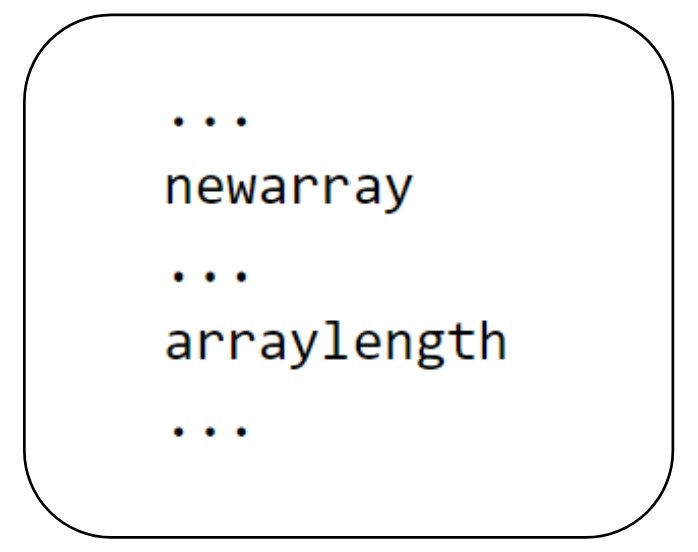
\includegraphics[scale=0.7]{bytecodes_array.jpg}
    \caption{Пример инструкций в программе}
\end{figure}

С другой стороны, каждый встроенный тип находит отражение в некотором C++-классе. При этом, при исполнении инструкции \textit{newarray} будет происходить аллокация экземпляра этого класса, а при исполнении \textit{arraylength} будет произведено чтение поля \textit{size\_} одного из экземпляров (рис. 2.2).

\begin{figure}[H]
    \centering
    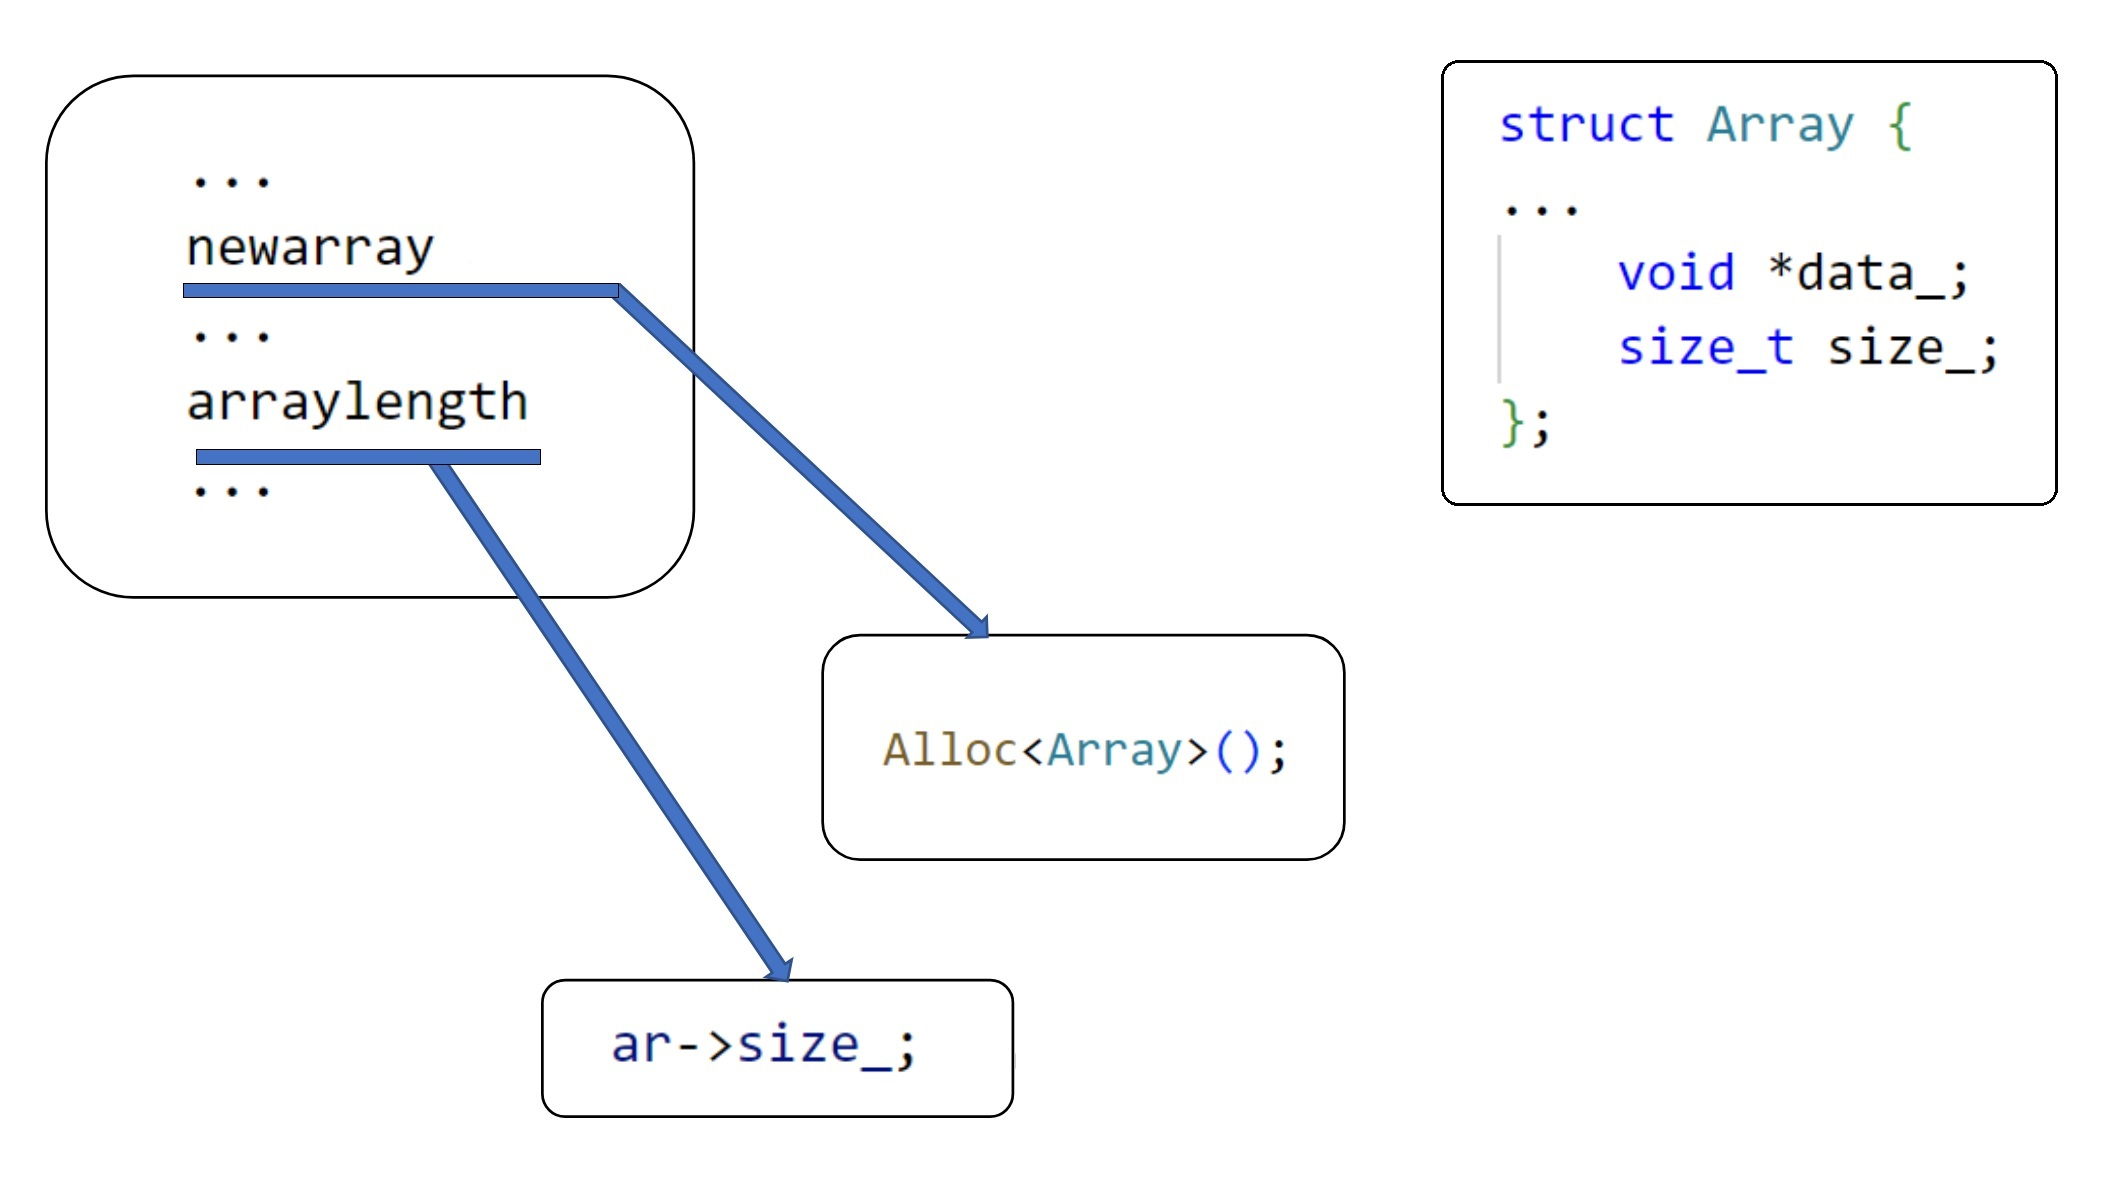
\includegraphics[scale=0.5]{mirror_class.jpg}
    \caption{Реализация семантики языка}
\end{figure}

В нативном формате, обращение к этому полю будет выражено в виде машинной инструкции загрузки по указателю с константным смещением.
Возвращаясь к кросс-компилятору виртуальной машины, эта инструкция будет создана на финальном этапе, кодогенерации, из соответствующей инструкции промежуточного представления.
Фактически, эта инструкция промежуточного представления абстрагирует бинарный формат машинной инструкции загрузки по смещению конкретной архитектуры, отделяя зависимость от платформы.
Однако, такой абстракции для отделения оказывается недостаточно.
Дело в том, что смещение до поля класса (эквивалентное в рассматриваемой ситуации смещению в инструкции загрузки), в общем случае, зависит от платформы.
Это может происходить по разным причнам, например -- из-за зависимости размера какого-либо элемента структуры данных от платформы, выравнивания по разным адресам.
Так, рассматриваемое ранее смещение до поля \textit{size\_} структуры \textit{Array} на 64-битной архитектуре AMD64 будет равно 8 байтам, хотя на архитектуре ARM32 -- 4.
Если упустить из рассмотрения этот факт, то кросс-компилятор виртуальной машины, запущенный на AMD64-сервере, при генерирации ARM32-инструкций будет использовать соответствующее текущей платформе значение смещения.
Тогда, при запуске такого кода на ARM32-телефоне, исполнение такой инструкции приведёт к некорректному поведению и является программной уязвимостью.
Вопрос корректности и безопасности генерируемого кода является первостепенным в процессе компиляции, что подчёркивает значимость этой проблемы.
Можно выделить два подхода, позволяющие разрешить этот конфликт: первый -- сделать смещения для всех платформ одинаковыми, второй -- каким-либо образом сообщать компилятору значение константы на платформе, для которой происходит компиляция. В следующей главе будет произведено сравнение этих подходов из которого становится ясным, почему предпочтение было отдано последнему из них. 

\newpage
